%! Author = Len Washington III
%! Date = 2/8/24

% Preamble
\documentclass[title={Chapter 5}]{fdsn201notes}

% Packages

% Document
\begin{document}

%<*Chapter5>
\maketitle{5}{Fats: Essential Energy-Supplying Nutrients}%

\section{What are Fats?}\label{sec:what-are-fats?}
\begin{itemize}
	\item Fats are one type of lipid
	\item \definition{Lipid}{diverse class of organic substances that are insoluble in water}
	\begin{itemize}
		\item Lipids (fats) do not dissolve in water
	\end{itemize}
\end{itemize}

\subsection{Triglycerides}\label{subsec:triglycerides}
\begin{itemize}
	\item Most of the fat we eat is in the form of triglycerides
	\begin{itemize}
		\item About 95\% of the fats we consume
	\end{itemize}
	\item Triglycerides are composed of
	\begin{itemize}
		\item Three fatty acid molecules
		\begin{itemize}
			\item \definition{Fatty acids}{long chains of carbon atoms surrounded by hydrogen atoms}
		\end{itemize}
		\item One glycerol molecule
		\begin{itemize}
			\item \definition{Glycerol}{a three-carbon alcohol that is the backbone of a triglyceride}
		\end{itemize}
	\end{itemize}
\end{itemize}

\begin{figure}[H]
	\centering
	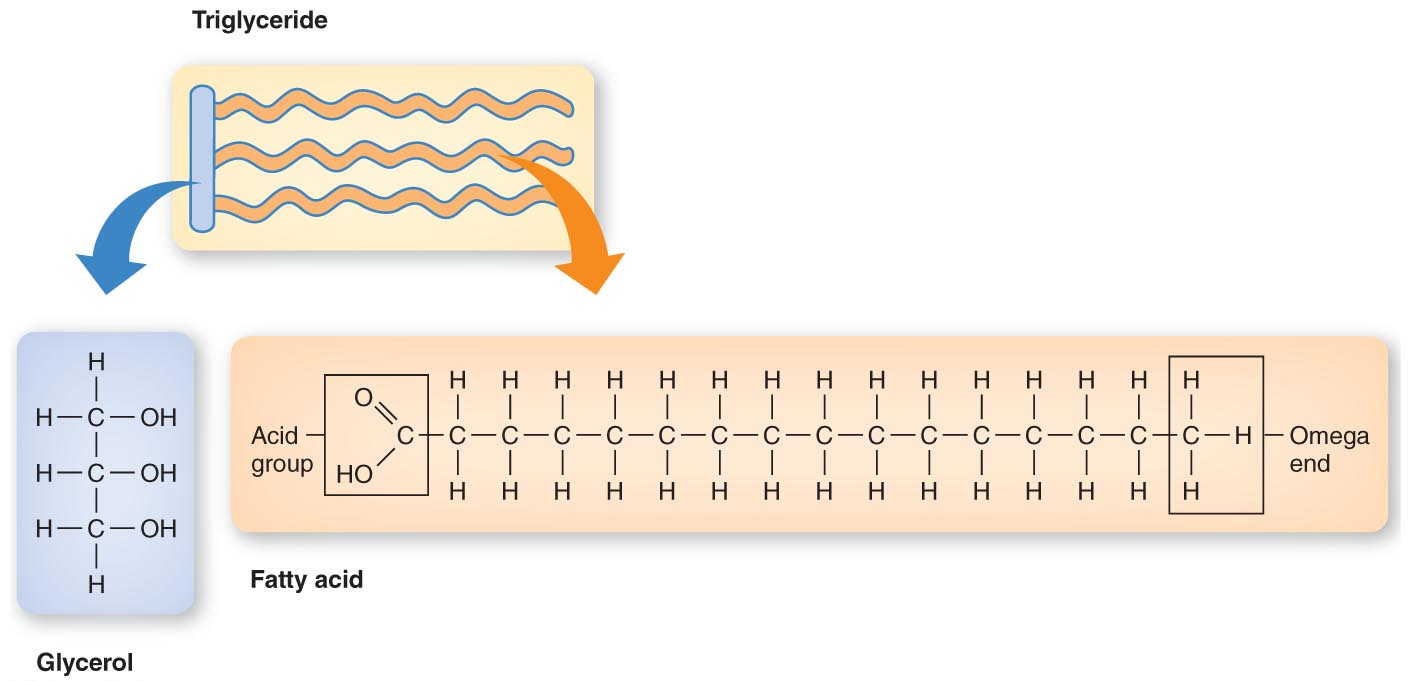
\includegraphics[width=\textwidth]{5_triglycerides}
	\caption{Triglyceride molecule}
	\label{fig:triglyceride}
\end{figure}

\subsection{Phospholipids}\label{subsec:phospholipids}
\begin{itemize}
	\item Composed of
	\begin{itemize}
		\item Glycerol backbone
		\item Two fatty acids
		\item Phosphate
	\end{itemize}
	\item Soluble in water
	\item Manufactured in our bodies so they are not required in our diet
	\item Important components of cell membranes
\end{itemize}

\subsection{Sterols}\label{subsec:sterols}
\definition{Sterols}{Lipids containing multiple rings of Carbon atoms}
\begin{itemize}
	\item Essential components of cell membranes and many hormones
	\item Manufactured in our bodies and therefore not an essential component of our body
	\item Cholesterool is the major sterol found in the body
\end{itemize}

\begin{figure}[H]
	\centering
	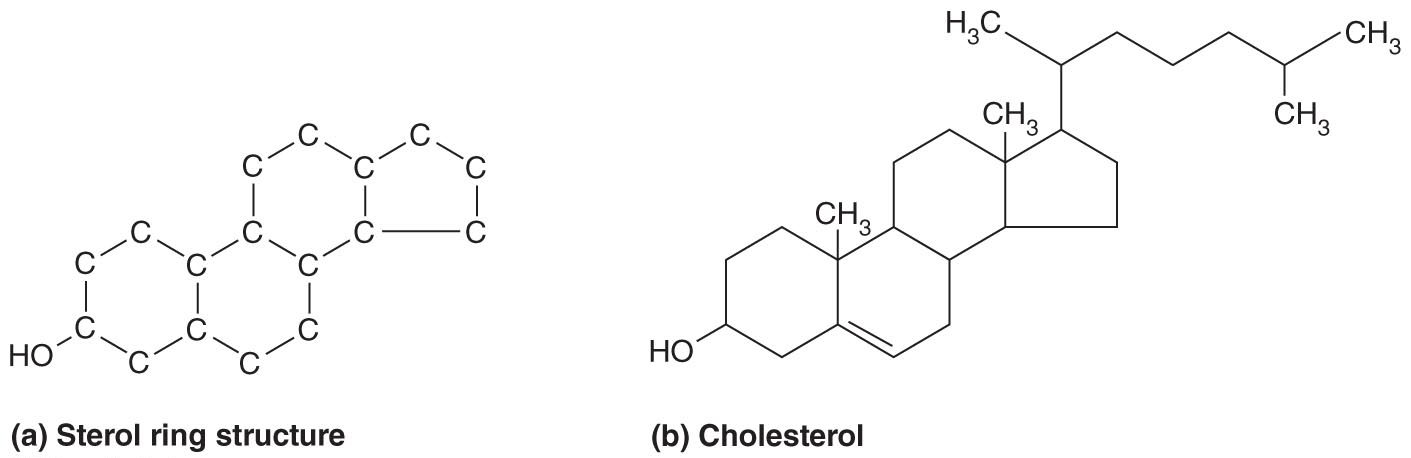
\includegraphics[width=\textwidth]{5_sterol}
	\caption{Sterol diagram}
	\label{fig:sterol}
\end{figure}

\begin{itemize}
	\item Fatty acids can differ in
	\begin{itemize}
		\item Length of their carbon chain
		\begin{itemize}
			\item Short ($<6$ Carbons)
			\item Medium ($6--12$ Carbons)
			\item Long ($>13$ Carbons)
		\end{itemize}
		\item Level of saturation
		\begin{itemize}
			\item Saturation refers to how many hydrogen atoms surround each carbon
		\end{itemize}
		\item Shape
	\end{itemize}
	\item \definition{Saturated fatty acids}{have strong hydrogen atoms surrounding every Carbon in the chain; they have no double bonds}
	\item \definition{Monosaturated fatty acids}{lack hydrogen atoms in one region; they have one double bond}
	\item \definition{Polysaturated fatty acids}{lack hydrogen atoms in multiple locationsl they have two or more double bonds}
	\item Note: Each double bond causes the loss of two hydrogen atoms
\end{itemize}

\begin{figure}[H]
	\centering
	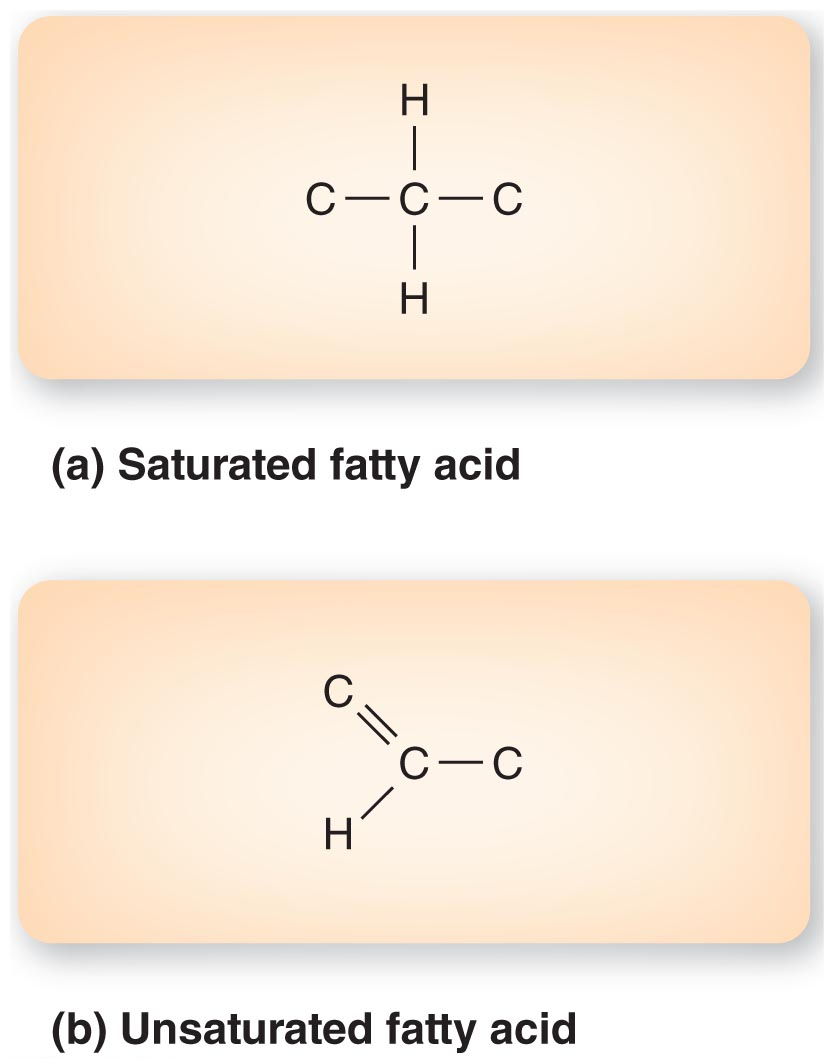
\includegraphics[width=\textwidth]{5_fatty_acids}
	\caption{Saturated and Unsaturated Fatty Acids}
	\label{fig:fatty-acids}
\end{figure}

\begin{figure}[H]
	\centering
	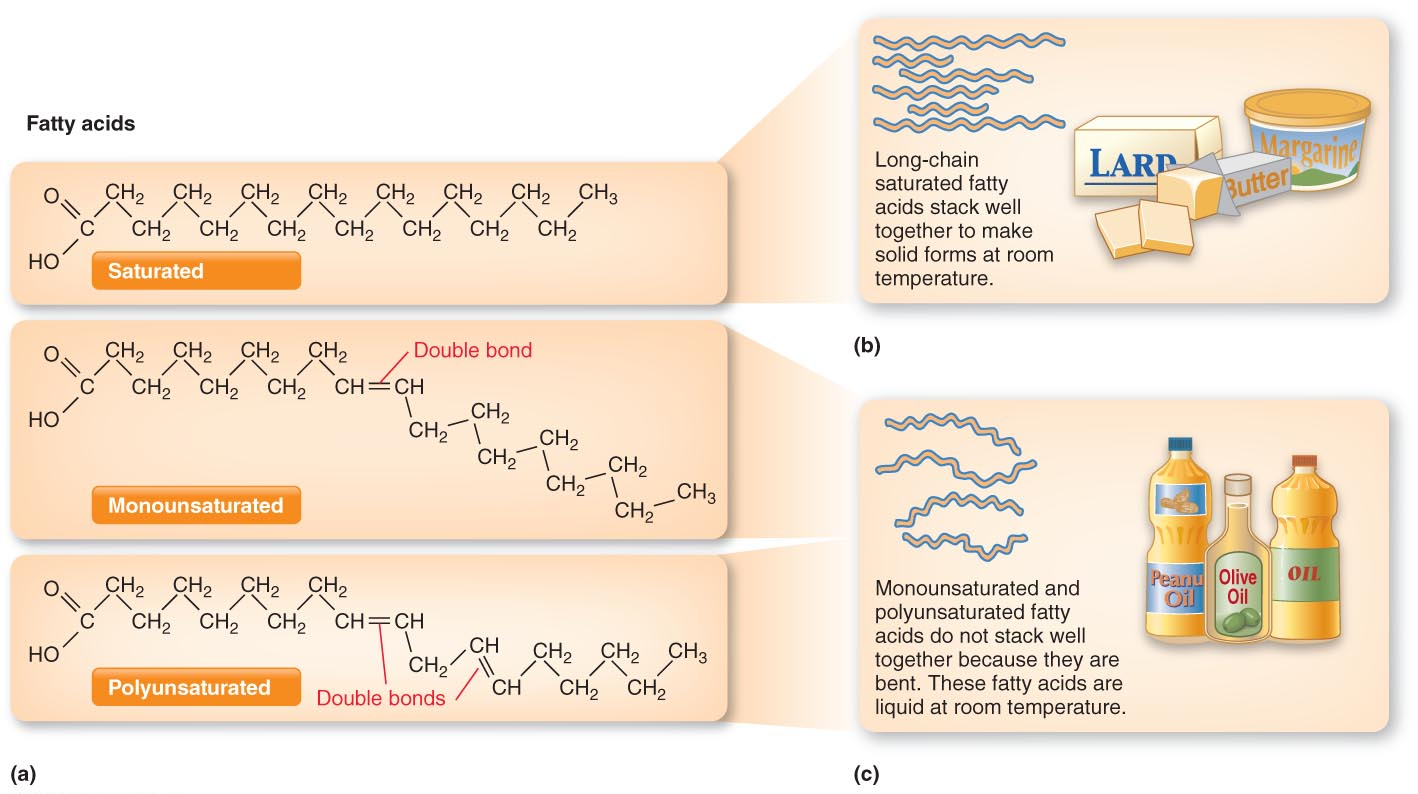
\includegraphics[width=\textwidth]{5_fatty_acid_levels}
	\caption{Levels of Saturation Among Fatty Acids}
	\label{fig:fatty-acid-saturation}
\end{figure}

\begin{figure}[H]
	\centering
	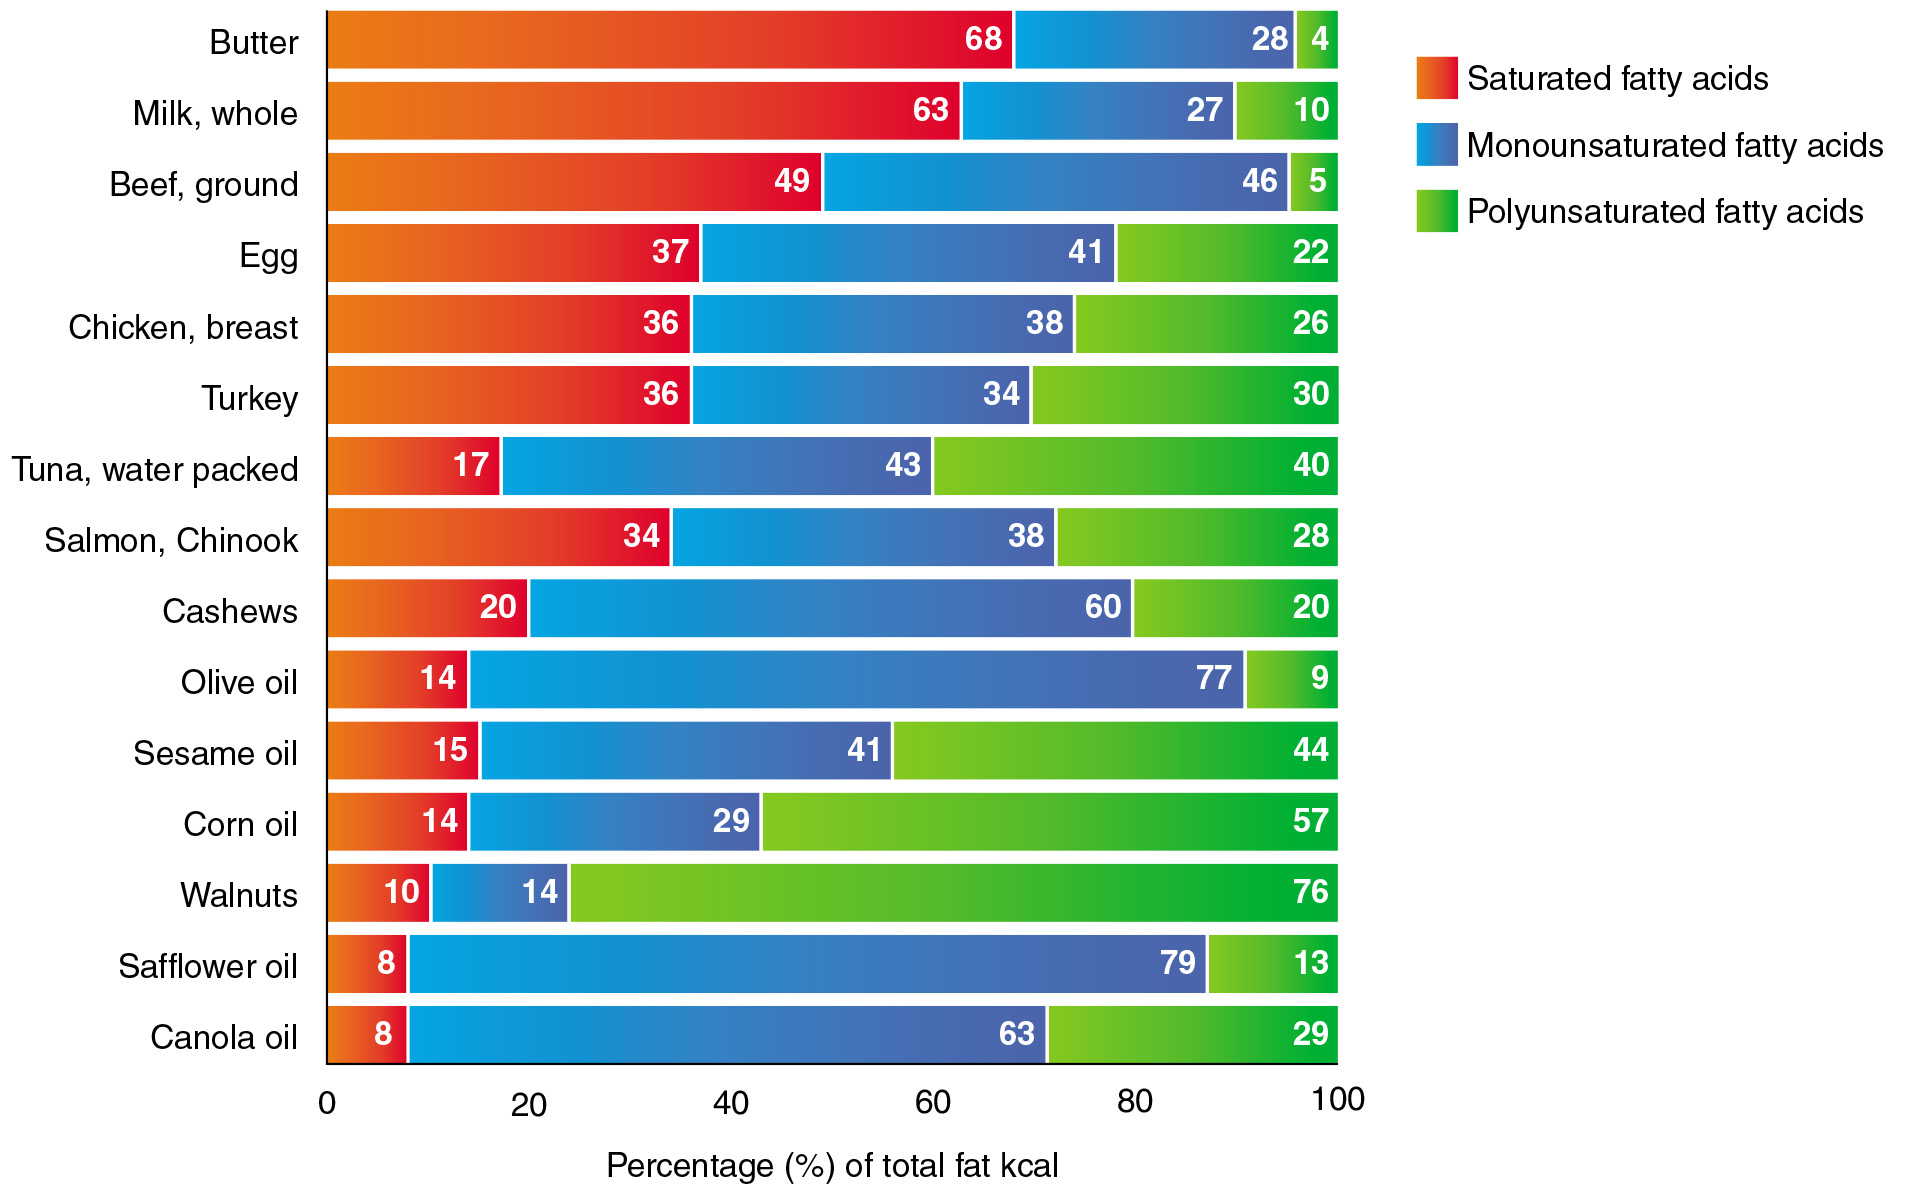
\includegraphics[width=\textwidth]{5_dietary_fat_sources}
	\caption{Major Sources of Dietary Fat}
	\label{fig:dietary_fat_sources}
\end{figure}

\begin{itemize}
	\item The shape of a triglyceride is determined by the saturation of the carbon chains
	\item Saturated fatty acids can pack tightly together and are solid at room temperature
	\begin{itemize}
		\item For example, coconut oil, animal fats, butter, and lard are high in saturated fatty acids
	\end{itemize}
	\item Unsaturated fatty acids do not stack together well and are liquid at room temperature
	\begin{itemize}
		\item Unsaturated fatty acids are the predominant type in plants
		\item Two exceptions are coconut and palm kernel oil
	\end{itemize}
	\item The hydrogen atoms at the unsaturated region can be arranged in different positions
	\begin{description}
		\item[Cis] same side of the carbon chain
		\item[Trans] opposite sides of the carbon chain
	\end{description}
\end{itemize}

\begin{itemize}
	\item \definition{Hydrogenation}{the addition of hydrogen atoms to unsaturated fatty acids}
	\begin{itemize}
		\item Converts liquid fats (oils) into a semisolid (spreadable) or solid form
		\item Used to create margarine from plant oil
		\item Often creates \emph{trans} fatty acids
		\item Listed on food labels as partially hydrogenated oil
	\end{itemize}
\end{itemize}

\section{Essential Fatty Acids}\label{sec:essential-fatty-acids}
\definition{Essential Fatty Acids}{cannot be synthesized in the body and must be obtained in the diet}
\begin{itemize}
	\item Omega-6 and omega-3 fatty acids
	\item There are precursors to biological compounds called \textit{eicosanoids}, which regulate cellular function
	\item Linoleic acid is found in vegetable and nut oils
	\item Alpha-linolenic acid (ALA) is derived from dark-green leafy vegetables, flaxseeds and flaxseed oil, soybeans and soybean oil, walnuts and walnut oil, and canola oil
	\item Eicosapentaenoic acid (EPA) and docosahexaenoic acid (DHA) have important health benefits and are found in fish, shellfish, and fish oils
\end{itemize}

\section{Why Do We Need Fats?}\label{sec:why-do-we-need-fats?}
\subsection{Energy}\label{subsec:energy}
\begin{itemize}
	\item Fat is very energy dense, providing 9 kcal/gram
	\item Much of the energy used during rest comes from fat
	\item Fat is used for energy during exercise, especially after glycogen is depleted
	\item Fat is also used for energy storage
\end{itemize}

\subsection{Fat-soluble vitamins}\label{subsec:fat-soluble-vitamins}
\begin{itemize}
	\item Vitamins A, D, E, and K are soluble in fat; fat is required for their transport
	\item Fat is essential to many body functions
	\begin{itemize}
		\item Cell membrane structure
		\item Nerve cell transmissions
		\item Protection of internal organs
		\item Insulation to retain body heat
	\end{itemize}
	\item Fat provides flavor and texture to foods
	\item Fat contributes to making us feel satiated
	\begin{itemize}
		\item Fats are more energy dense than carbohydrates or protein
		\item Fats take longer to digest
	\end{itemize}
\end{itemize}

\section{How Does Our Body Process Fats?}\label{sec:how-does-our-body-process-fats?}
\begin{itemize}
	\item As fat enters the small intestine:
	\begin{itemize}
		\item Bile is secreted from the gallbladder into the small intestine
		\begin{itemize}
			\item Bile is produced by the liver and stored in the gallbladder
		\end{itemize}
		\item Bile disperses dat into smaller fat droplets
		\item Pancreatic enzymes break triglycerides into two separate fatty acids and a monoglyceride
		\item Fat enters the mucosal cell as a micelle (fatty acids, monoglycerides), phospholipids, and sterols)
	\end{itemize}
	\item In the intestinal mucosal cell:
	\begin{itemize}
		\item Fatty acids are reattached to the monoglyceride to re-form triglycerides
		\item A small amount of protein is added to lipids, forming a chylomicron
		\item \definition{Chylomicron}{a lipoprotein produced by cells lining the small intestine}
		\begin{itemize}
			\item Composed of triglycerides surrounded by phospholipids and proteins
			\item Soluble in water
		\end{itemize}
	\end{itemize}
	\item Chylomicrons are the transport vehicles that remove absorbed fats from the small intestine
	\begin{itemize}
		\item Travel through the lymphatic system
		\item Are transferred to the bloodstream
	\end{itemize}
	\item Short- and medium-chain fatty acids are absorbed more quickly because they are not arranged into chylomicrons
	\item Once the chylomicron gets to a cell in the body, the triglycerides in the chylomicrons must be disassembled by lipoprotein lipase into two fatty acids and a monoglyceride before they can pass through the cell membrane
	\item After entering the cell, the two fatty acids and monoglyceride re-form a triglyceride
	\item The triglyceride can be
	\begin{itemize}
		\item Used immediately for energy
		\item Used to make lipid-containing compounds
		\item Stored in liver and muscle cells
	\end{itemize}
\end{itemize}

\section{Recognize the Fat in Foods}\label{sec:recognize-the-fat-in-foods}
\begin{description}
	\item[Visible fats] those we can see in foods or can easily see have been added to foods, such as dressing or chicken skin
	\item[Hidden fats] those added to processed or prepared foods to improve texture or taste, which we may not be aware of, or that occur naturally
\end{description}
\begin{itemize}
	\item Read the Nutrition Facts Panel on foods carefully
	\begin{itemize}
		\item Lower-fat versions of foods may not always be lower in Calories
	\end{itemize}
\end{itemize}

\section{How Much Fat Should We Eat?}\label{sec:how-much-fat-should-we-eat?}
\begin{itemize}
	\item The Acceptable Macronutrient Distribution Range (AMDR) for fat
	\begin{itemize}
		\item 20--35\% of Calories should be from fat
	\end{itemize}
	\item Athletes and highly active people may need more energy from carbohydrates and can reduce their fat intake to 20--25\% of total Calories
	\item The type of fat consumed is important
	\begin{itemize}
		\item Intake of saturated and \textit{trans} fatty acids should be minimized as much as possible
		\item We typically set enough linoleic acid in our diets from salad dressings, vegetable oils, margarines, and mayonnaise
		\item To ensure an adequate amount of omega-3 fatty acids, we need to consume more dark-green leafy vegetables, walnuts, flaxseeds, and fish or fish oils
	\end{itemize}
\end{itemize}

\section{Essential Fatty Acids}\label{sec:essential-fatty-acids-2}
\begin{itemize}
	\item Linoleic Acid (omega-6)
	\begin{itemize}
		\item AI is 14--17 g per day for men and 11--12 g per day for women
	\end{itemize}
	\item Alpha-linoleic acid (Omega-3)
	\begin{itemize}
		\item AI is 1.6 g per day for men and 1.1 g per day for women
	\end{itemize}
\end{itemize}

\section{Limit Saturated and \textit{Trans} Fats}\label{sec:limit-saturated-and-trans-fats}
\begin{itemize}
	\item Reduce your intake of saturated fats
	\begin{itemize}
		\item Be conscious of the saturated fat content of meats, baked goods and snack goods, and foods including vegetables that are fried, breaded, or drenched in sauce
	\end{itemize}
	\item Avoids \textit{trans} fatty acids
	\item Limit your intake of dietary cholesterol, which will also help limit your intake of saturated fats
\end{itemize}

\section{Select Beneficial Fats}\label{sec:select-beneficial-fats}
\begin{itemize}
	\item Consume and cook with leafy green vegetables, avocados, soybeans, soybean oil, and flaxseed oil
	\item Add walnuts, almonds, flaxseeds, and chia seeds to your diet, and try almond milk in your cereal
	\item Consider including fish in your diet at least twice a week or consider taking a fish oil supplement
	\begin{itemize}
		\item Fish can contain mercury, PCBs, and other environmental contaminants, so be selective
	\end{itemize}
\end{itemize}

\section{Fat Replacers}\label{sec:fat-replacers}
\begin{itemize}
	\item Snack foods are frequent targets for fat replacers, substances that can reduce the fat content
	\item Fat replacers such as olestra have not proved very popular or effective because of potential gastrointestinal side effects
	\item Our growing obesity problems indicate that fat replacers do not help Americans lose weight
\end{itemize}

\section{Role of Fats in Chronic Disease}\label{sec:role-of-fats-in-chronic-disease}
\begin{itemize}
	\item The chronic disease most closely associated with diets high in saturated fat is cardiovascular disease
	\item The role of dietary fat in the development of cancer has been extensively researched, but the relationship between some cancer types and dietary fats is controversial (e.g., breast cancer)
	\item The strongest association between dietary fat and cancer is for prostate cancer
\end{itemize}

\section{In Depth: Cardiovascular Disease (CVD)}\label{sec:in-depth:-cardiovascular-disease}
\begin{itemize}
	\item Dysfunction of the heart or blood vessels
	\item The most common forms:
	\begin{itemize}
		\item Coronary heart disease, or coronary artery disease
		\item Stroke
		\item Hypertension, or high blood pressure
		\item Peripheral vascular disease
	\end{itemize}
	\item \definition{Atherosclerosis}{a disease in which artery walls build up lipid deposits and scar tissue, impairing blood flow}
	\begin{itemize}
		\item The stiffness that results is commonly called ``hardening of the arteries''
		\item The result is that the heart must work harder to push blood through the vessels
	\end{itemize}
	\item \definition{Hypertension}{a major chronic disease in the United States}
	\begin{itemize}
		\item It functions as a warning sign for a person's risk for developing heart disease or stroke
		\item For many people, hypertension is hereditary; for others, it can be induced through poor nutrition and exercise habits or a combination of poor habits and heredity
	\end{itemize}
	\item Modifiable risk factors for cardiovascular disease include
	\begin{itemize}
		\item Being overweight
		\item Physical inactivity
		\item Smoking
		\item Type 2 diabetes mellitus
		\item Inflammation in the body
		\item Abnormal blood lipids
	\end{itemize}
	\item The intake of certain types of fats can protect against heart disease
	\item Diets high in omega-3 fatty acids (along with moderate exercise) can reduce inflammation and increase HDL (``good'') cholesterol levels
	\item Low-density lipoproteins (LDLs) are often called ``bad'' cholesterol because of their role in transporting cholesterol throughout the body
	\item Diets high in saturated fats
	\begin{itemize}
		\item Decrease the removal of LDLs from the blood
		\item Contribute to the formation of plaques that can block arteries
		\item Increase triglyceride levels (chylomicrons and very-low-density lipoproteins, or VLDLs)
	\end{itemize}
	\item Recommendations to improve blood lipid levels
	\begin{itemize}
		\item Keep total fat intake level to within 20--35\% of your daily energy intake
		\item Decrease your dietary saturated fat to less than 7\% of total energy intake
		\item Increase your consumption of dietary omega-3 fatty acids from foods (e.g., green vegetables, fish)
		\item Consume 400 $\mu$g/day of folate
		\item Increase dietary intakes of whole grains, fruits and vegetables
		\item Maintain blood glucose within normal ranges
		\item Eat meals throughout the day rather than eating most of your Calories in the evening before bed
		\item Limit alcohol consumption
		\item Don't smoke
		\item Maintain an active lifestyle
		\item Maintain a healthful body weight
	\end{itemize}
	\item Recommendations to reduce blood pressure
	\begin{itemize}
		\item Limit dietary sodium
		\item Follow the DASH diet ``Dietary Approaches to Stop Hypertension''
		\item If need, use doctor-prescribed medications
	\end{itemize}
\end{itemize}

%</Chapter5>

\end{document}
